% LAST CHANGES BY RN 26/10/15
% Submitted to Int. J. Numer. Methods Fluids on 26/10/15.
\documentclass[a4paper,12pt,onecolumn]{article}

\usepackage[utf8]{inputenc}
\usepackage[english]{babel}
\usepackage{amssymb,amsmath,amsthm,array,epsfig,pstricks,subfig,hyperref,verbatim}

\newtheorem{thm}{Theorem}
\newtheorem{lem}[thm]{Lemma}
\newtheorem{rem}[thm]{Remark}

\newenvironment{keywords}{{\upshape\bfseries Key words. }\ignorespaces}{}

\newcommand{\R}{{\mathbb R}}
\newcommand{\vol}{\mathcal{L}^d}
\newcommand{\dH}[1]{\;{\rm d}{\cal H}^{#1}} % Hausdorff measure
\newcommand{\dL}[1]{\;{\rm d}{\cal L}^{#1}} % Lebesgue measure
\newcommand{\bigchi}{\ensuremath{\mathrm{\mathcal{X}}}}
\newcommand{\charfcn}[1]{\bigchi_{#1}} % characteristic function
\newcommand{\Vh}{\underline{V}(\Gamma^m)}
\newcommand{\Wh}{W(\Gamma^m)}
\newcommand{\Vht}{\underline{V}(\Gamma^h(t))}
\newcommand{\Wht}{W(\Gamma^h(t))}
\newcommand{\uspace}{\mathbb{U}}
\newcommand{\pspace}{\mathbb{P}}
\newcommand{\kspace}{\mathbb{K}}
\newcommand{\xspace}{\mathbb{X}}
\newcommand{\sigmaO}{o}
\newcommand{\nabs}{\nabla_{\!s}}
\newcommand{\id}{\rm id}
\newcommand{\ddt}{\frac{\rm d}{{\rm d}t}}
\newcommand{\NbulkT}{\vec{N}_{\Gamma,\Omega}^T}
\newcommand{\Nbulk}{\vec{N}_{\Gamma,\Omega}}
\newcommand{\errorXx}{\|\Gamma^h - \Gamma\|_{L^\infty}}
\newcommand{\errorUu}[1]{\|\vec U - I^h_{#1}\,\vec u\|_{L^\infty}}
\newcommand{\LerrorPp}{\|P - p\|_{L^2(\Omega_T)}}
\newcommand{\unitn}{\vec{\rm n}}
\newcommand{\mat}[1]{\underline{\underline{#1}}\rule{0pt}{0pt}}

\renewcommand{\theequation}{\arabic{section}.\arabic{equation}}

\textwidth 425pt

\title{Fitted Finite Element Discretization of \\ Two--Phase Stokes Flow}
\author{Marco Agnese and Robert N\"urnberg%
\thanks{email: \texttt{\{m.agnese13,robert.nurnberg\}@imperial.ac.uk}}\\
\small
Department of Mathematics, Imperial College, London, SW7 2AZ, U.K.}
\date{}

\begin{document}

\captionsetup[subfigure]{labelformat=empty} % remove label subplot

\maketitle

\begin{abstract}
We propose a novel fitted finite element method for two-phase Stokes
flow problems that uses piecewise linear finite elements to approximate the
moving interface. The method can be shown to be unconditionally stable.
Moreover, spherical stationary solutions are captured exactly by the numerical
approximation. In addition, the meshes describing the discrete interface in
general do not deteriorate in time, which means that in numerical simulations a
smoothing or a remeshing of the interface mesh is not necessary.
We present several numerical experiments for our numerical method, which
demonstrate the accuracy and robustness of the proposed algorithm.
\end{abstract}

\begin{keywords}
viscous incompressible two-phase flow, Stokes equations,
free boundary problem, surface tension, finite elements, front tracking
\end{keywords}

\section{Introduction}\label{sec:introduction}
Fluid flow problems with a moving interface are encountered in many
applications in physics, engineering and biophysics. Developing robust and
efficient numerical methods for these flows is an important problem and
has attracted tremendous interest over the last decade. Apart from the usual
difficulties arising from the numerical computation of the fluid flow in the
bulk, the accurate approximation of the moving free interface, as well as a
suitable description of the conditions that need to hold on the interface,
pose serious challenges. Of particular importance is the precise inclusion of
surface tension terms, and the correct handling of discontinuity jumps in the
material properties and in the pressure at the interface, in order to suppress
spurious velocities, which are also called parasitic currents.

In this paper we propose a novel finite element approximation for
incompressible two-phase Stokes flow that naturally avoids spurious
velocities. Our scheme is based on the numerical method introduced in
\cite{spurious}, and so uses piecewise linear parametric finite elements to
describe the moving discrete interface. In contrast to \cite{spurious}, where
the interface and the bulk mesh were totally independent, here we pursue the
fitted approach. That means that the interface discretization is always fitted
to the bulk mesh, i.e.\ the discrete interface is made up of edges/faces of
elements belonging to the bulk mesh. An advantage of our method is that the
discontinuity jumps in the material properties and in the pressure are captured
naturally. In particular, we do not need to employ an XFEM-type extension of
standard bulk pressure spaces. Surface tension forces are discretized with the
help of a variational approximation of curvature that was first proposed in
\cite{triplej,gflows3d}. Combining this was an implicit treatment of the
surface tension forces yields an unconditionally stable scheme. Interestingly,
the formulation of curvature from \cite{triplej} leads to a tangential motion
of vertices in practice, which guarantees equidistribution in 2d and good
meshes in 3d. Overall, our proposed method has the following properties.
\begin{itemize}
\item The fully discrete scheme is unconditionally stable in the sense that the
total surface energy is monotonically decreasing independent of the chosen time
step size.
\item In the absence of outer forces, any discrete solution with a stationary
interface must have zero velocity globally, i.e.\ we can prove that there are
no stationary solutions with spurious velocities. Similarly, discrete
stationary solutions for spherical interfaces are attained for our scheme.
\item For the semidiscrete continuous-in-time variant of the fully discrete
scheme the volume
of the two phases is conserved. The fully discrete scheme itself maintains the
enclosed volumes well in practice.
\item Thanks to the fitted nature of the finite element method, the pressure
jumps at the interface are captured accurately for standard pressure finite
element spaces without the need for XFEM extensions.
\item The surface tension effects are included with the help of a variational
treatment of curvature based on the Laplace--Beltrami operator.
\item The surface mesh quality is maintained. In particular, for the
semidiscrete scheme an equidistribution property can be shown in 2d.
\item The fully discrete scheme uses an implicit approximation of curvature
that leads to a coupled linear system of equations to be solved at each time
step.
\end{itemize}

Let us briefly discuss alternative approaches to the numerical approximation of
two-phase flow problems. In this paper we use a direct description of the
interface.  In such direct
approaches, which are often called front-tracking methods, the interface is
either triangulated or presented by a connected set of particles. The discrete
interface is advected with the help of the bulk fluid velocities, and
quantities on the interface need to be suitably coupled to the bulk equations.
In our situation, a finite element parameterization of the unknown interface
is employed.
We refer e.g.\ to
\cite{UnverdiT92,Bansch01,Tryggvason_etal01,GanesanMT07,GanesanT08,spurious}
for further details on front tracking methods,
and to \cite{LevequeL97,Peskin02} for the related immersed
boundary method. Another class of approaches is based on interface capturing
methods using an indicator function to describe the interface. The volume of
fluid (VOF) method and the level set method fall into this category. In the
former, the characteristic function of one of the phases is approximated
numerically, see e.g.\ \cite{HirtN81,RenardyR02,Popinet09}; whereas in the
latter, the interface is given as the level set of a function, which has to be
determined, see e.g.\ \cite{SussmanSO94,Sethian99,OsherF03,GrossR07}.
Finally, in phase
field methods the interface is assumed to have a small, but positive, thickness
and an additional parabolic equation, defined in the whole domain, has to be
solved in these so-called diffuse interface models. We refer to
\cite{HohenbergH77,AndersonMW98,LowengrubT98,Feng06,KaySW08,AbelsGG12,GrunK14}
for details.

The remainder of this paper is organized as follows. In Section~\ref{sec:2}
we present the mathematical model and the weak formulation on which our finite
element approximation is going to be based. Our numerical method is presented
in Section~\ref{sec:3}, together with proofs for its main properties. In
addition, we describe how the arising linear systems of equations are solved in
practice, and we give details on our mesh generation and smoothing procedures.
Finally, in Section~\ref{sec:4} we present several numerical simulations in 2d
and 3d.

\section{Mathematical model} \label{sec:2}

\subsection{Governing equations}
In this paper we consider two--phase Stokes flow in a given domain
$\Omega\subset\mathbb{R}^d$, where $d=2$ or $d=3$. The domain $\Omega$ contains
two different immiscible, incompressible, viscous fluids (liquid-liquid or
liquid-gas) which for all $t\in[0,T]$ occupy time dependent regions
$\Omega_+(t)$ and $\Omega_-(t):=\Omega\setminus\overline{\Omega}_+(t)$ and
which are separated by an interface
$(\Gamma(t))_{t\in[0,T]}$, $\Gamma(t)\subset\Omega$.
See Figure~\ref{fig:sketch} for an illustration.
\begin{figure}
\begin{center}
\unitlength15mm
\psset{unit=\unitlength,linewidth=1pt}
\begin{picture}(4,4)(0,0)
\psline(0,0)(4,0)(4,4)(0,4)(0,0)
\psellipse(2,2)(1,1)
\psline{->}(3,2)(3.5,2)
\put(3.25,1.75){$\vec\nu$}
\put(1.75,0.75){{$\Gamma(t)$}}
\put(1.75,2){{$\Omega_-(t)$}}
\put(0.5,3.25){{$\Omega_+(t)$}}
\end{picture}
\end{center}
\caption{The domain $\Omega$ in the case $d=2$.}
\label{fig:sketch}
\end{figure}
For later use, we assume that $(\Gamma(t))_{t\in [0,T]}$ is a sufficiently
smooth evolving hypersurface without boundary that is parameterized by
$\vec x(\cdot,t):\Upsilon\to\R^d$, where $\Upsilon\subset \R^d$ is a given
reference manifold, i.e.\ $\Gamma(t) = \vec x(\Upsilon,t)$. Then
\begin{equation} \label{eq:V}
\vec{\mathcal{V}}(\vec z, t) := \vec x_t(\vec q, t) \qquad
\forall\ \vec z = \vec x(\vec q,t) \in \Gamma(t)
\end{equation}
defines the velocity of $\Gamma(t)$, and $\vec{\mathcal{V}} \,.\,\vec{\nu}$ is
the normal velocity of the evolving hypersurface $\Gamma(t)$,
where $\vec\nu(t)$ is the unit normal on $\Gamma(t)$ pointing into
$\Omega_+(t)$.

Denoting the velocity and pressure by $\vec u$ and $p$, respectively, we
introduce the stress tensor
\begin{equation} \label{eq:stress_tensor}
\mat\sigma = \mu \,(\nabla\,\vec u + (\nabla\,\vec u)^T) - p\,\mat\id
= 2\,\mu\, \mat D(\vec u)-p\,\mat\id\,,
\end{equation}
where $\mu(t) = \mu_+\,\charfcn{\Omega_+(t)} + \mu_-\,\charfcn{\Omega_-(t)}$,
with $\mu_\pm \in \R_{>0}$, denotes the dynamic viscosities in the two phases,
$\mat\id \in \R^{d \times d}$ is the identity matrix and
$\mat D(\vec u):=\frac12\, (\nabla\vec u+(\nabla\vec u)^T)$
is the rate-of-deformation tensor.

In this paper we consider a two-phase Stokes problem, and so the equations
governing the fluid are
\begin{subequations}
\begin{alignat}{2}
- \nabla\,.\,\mat\sigma & = \vec f \qquad &&\mbox{in } \Omega_\pm(t)\,,
\label{eq:stokes_momentum} \\
\nabla\,.\,\vec u & = 0 \qquad &&\mbox{in } \Omega_\pm(t)\,,
\label{eq:stokes_mass}
\end{alignat}
\end{subequations}
where $\vec f$ is a possible forcing term.

On the free surface $\Gamma(t)$, the following conditions need to hold:
\begin{subequations}
\begin{alignat}{2}
[\vec u]_-^+ & = \vec 0 \qquad &&\mbox{on } \Gamma(t)\,,
\label{eq:interface_jump_velocity} \\
[\mat\sigma\,\vec \nu]_-^+ & = -\gamma\,\varkappa\,\vec\nu \qquad
&&\mbox{on } \Gamma(t)\,, \label{eq:interface_jump_stress} \\
\vec{\mathcal{V}}\,.\,\vec\nu &= \vec u\,.\,\vec \nu \qquad
&&\mbox{on } \Gamma(t)\,, \label{eq:interface_velocity}
\end{alignat}
\end{subequations}
where $\gamma>0$ is the surface tension coefficient and $\varkappa$ denotes the
mean curvature of $\Gamma(t)$, i.e.\ the sum of the principal curvatures of
$\Gamma(t)$, where we have adopted the sign convention that $\varkappa$ is
negative where $\Omega_-(t)$ is locally convex. In particular,
see e.g.\ \cite{DeckelnickDE05}, it holds that
\begin{equation} \label{eq:LBop}
\Delta_s\, \vec \id = \varkappa\, \vec\nu \qquad \mbox{on $\Gamma(t)$}\,,
\end{equation}
where $\Delta_s = \nabs\,.\,\nabs$ is the Laplace--Beltrami operator on
$\Gamma(t)$ with $\nabs\,.\,$ and $\nabs$ denoting surface divergence and
surface gradient on $\Gamma(t)$, respectively. Moreover, as usual,
$[\vec u]_-^+ := \vec u_+ - \vec u_-$ and
$[\mat\sigma\,\vec\nu]_-^+ := \mat\sigma_+\,\vec\nu - \mat\sigma_-\,\vec\nu$
denote the jumps in velocity and normal stress across the interface
$\Gamma(t)$. Here and throughout, we employ the shorthand notation
$\vec g_\pm := \vec g\!\mid_{\Omega_\pm(t)}$ for a function
$\vec g : \Omega \times [0,T] \to \R^d$; and similarly for scalar and
matrix-valued functions. To close the system we prescribe the initial data
$\Gamma(0) = \Gamma_0$ and the boundary condition $\vec u = \vec 0$ on
$\partial \Omega$.

Therefore the total system can be rewritten as follows:
\begin{subequations}
\begin{alignat}{2}
-2 \mu\,\nabla\,.\,\mat D(\vec u)+ \nabla\,p & = \vec f
\quad &&\mbox{in } \Omega_\pm(t)\,, \label{eq:full_momentum} \\
\nabla\,.\,\vec u & = 0 \quad &&\mbox{in } \Omega_\pm(t)\,,
\label{eq:full_mass} \\
\vec u & = \vec 0 \qquad &&\mbox{on } \partial\Omega\,,
\label{eq:full_initial_velocity} \\
[\vec u]_-^+ & = \vec 0 \quad &&\mbox{on } \Gamma(t)\,,
\label{eq:full_jump_velocity} \\
[2\mu \,\mat D(\vec u)\,.\,\vec\nu - p\,\vec \nu]_-^+
& = -\gamma\,\varkappa\,\vec\nu
\quad &&\mbox{on } \Gamma(t)\,, \label{eq:full_jump_stress} \\
(\vec{\mathcal{V}}-\vec u)\,.\,\vec{\nu} & = 0
\quad &&\mbox{on } \Gamma(t)\,,\label{eq:full_velocity}  \\
\Gamma(0) & = \Gamma_0 \,.\label{eq:full_initial_interface}
\end{alignat}
\end{subequations}

\subsection{Weak formulation}
In order to obtain a weak formulation, we define the function spaces
\begin{align*}
\uspace &:= H^1_0(\Omega, \R^d)\,,\qquad \pspace := L^2(\Omega) \qquad
\mbox{and}\qquad
\widehat\pspace := \{\eta\in\pspace : \int_\Omega\eta\dL{d}=0 \}\,,
\end{align*}
and let $(\cdot,\cdot)$ and $\langle \cdot, \cdot \rangle_{\Gamma(t)}$ denote
the $L^2$--inner products on $\Omega$ and $\Gamma(t)$, respectively. In
addition, we let $\mathcal{L}^d$ and $\mathcal{H}^{d-1}$ denote the Lebesgue
measure in $\R^d$ and the $(d-1)$-dimensional Hausdorff measure, respectively.

Multiplying (\ref{eq:LBop}) with a test function, and performing integration by
parts, yields
$$
\left\langle \varkappa\,\vec\nu, \vec\eta \right\rangle_{\Gamma(t)}
+ \left\langle \nabs\,\vec \id, \nabs\,\vec \eta \right\rangle_{\Gamma(t)}
= 0  \quad \forall\ \vec\eta \in [H^1(\Gamma(t)]^d\,.
$$
Moreover, on noting (\ref{eq:stress_tensor}) and (\ref{eq:full_jump_stress}),
we have that
\begin{align*}
\int_{\Omega_+(t)\cup\Omega_-(t)} (\nabla\,.\,\mat\sigma)\,.\, \vec \xi \dL{d}
& = - \left(\mat\sigma, \nabla\,\vec \xi\right)
- \left\langle [\mat\sigma\,\vec\nu]_-^+ , \vec \xi
  \right\rangle_{\Gamma(t)} \nonumber \\
& = \left( p , \nabla\,.\,\vec \xi\right)
-2 \left(\mu\,\mat D(\vec u) , \mat D(\vec \xi) \right)
+ \gamma \left\langle \varkappa\,\vec \nu , \vec \xi  \right\rangle_{\Gamma(t)}
\end{align*}
for all $\vec \xi \in [H^1_0(\Omega)]^d$. Hence a possible weak formulation of
(\ref{eq:full_momentum}--g) is given as follows. Given $\Gamma(0) = \Gamma_0$,
for almost all $t\in(0,T)$ find $\Gamma(t)$ and functions
$\vec u \in \uspace$, $p \in \widehat\pspace$, $\varkappa \in H^1(\Gamma(t))$
such that
\begin{subequations}
\begin{align}
& 2\left(\mu\,\mat D(\vec u), \mat D(\vec \xi)\right)
- \left(p, \nabla\,.\,\vec \xi\right)
- \gamma\,\left\langle \varkappa\,\vec\nu, \vec\xi\right\rangle_{\Gamma(t)}
= \left(\vec f, \vec \xi\right)\quad \forall\ \vec\xi \in \uspace \,,
\label{eq:weaka}\\
& \left(\nabla\,.\,\vec u, \varphi\right) = 0
\quad \forall\ \varphi \in \widehat\pspace\,, \label{eq:weakb} \\
&  \left\langle \vec{\mathcal{V}}
- \vec u, \chi\,\vec\nu \right\rangle_{\Gamma(t)} = 0
\quad \forall\ \chi \in H^1(\Gamma(t))\,, \label{eq:weakc} \\
& \left\langle \varkappa\,\vec\nu, \vec\eta \right\rangle_{\Gamma(t)}
+ \left\langle \nabs\,\vec \id, \nabs\,\vec \eta \right\rangle_{\Gamma(t)}
= 0  \quad \forall\ \vec\eta \in [H^1(\Gamma(t))]^d\,\label{eq:weakd}
\end{align}
\end{subequations}
holds for almost all times $t \in (0,T]$. Here we have observed that if
$p \in \pspace$ is part of a solution to (\ref{eq:full_momentum}--g), then so is
$p + c$ for an arbitrary $c\in \R$.

\subsection{Energy bound and volume conservation}
It is straightforward to show an a priori energy bound and a volume
conservation property for the system (\ref{eq:weaka}--d). For the former, we
recall from e.g.\ \cite[Lemma~2.1]{DeckelnickDE05} that
\begin{equation}\label{eq:dtarea}
\ddt\,\mathcal{H}^{d-1}(\Gamma(t)) = -
\left\langle \varkappa,\vec{\mathcal{V}}\,.\,\vec\nu\right\rangle_{\Gamma(t)}.
\end{equation}
Hence, on choosing $\vec\xi = \vec u$ in (\ref{eq:weaka}), and noting
(\ref{eq:weakb},c), we obtain that
\begin{align}
\gamma\, \ddt\,\mathcal{H}^{d-1}(\Gamma(t)) = -
\gamma\,\left\langle \varkappa\,\vec\nu, \vec u\right\rangle_{\Gamma(t)}
=  - 2\left(\mu\,\mat D(\vec u), \mat D(\vec u)\right) +
\left(\vec f, \vec u\right) \,,
\label{eq:ap1}
\end{align}
and so in the absence of outer forces, the interfacial energy is monotonically
decreasing.

In order to show the volume conservation property, we recall from e.g.\
\cite[Lemma~2.1]{DeckelnickDE05} that
\begin{align}
\ddt \vol(\Omega_-(t)) & = \left\langle \vec{\mathcal{V}}, \vec\nu
\right\rangle_{\Gamma(t)}\,.
\end{align}
Hence it follows immediately from the incompressibility condition
(\ref{eq:weakb}) and (\ref{eq:weakc}) that
\begin{align}
\ddt \vol(\Omega_-(t)) & = \left\langle \vec u , \vec\nu
\right\rangle_{\Gamma(t)}
 = \int_{\Omega_-(t)} \nabla\,.\,\vec u \dL{d} =0\,. \label{eq:conserved}
\end{align}
It will be our aim to introduce a fitted finite element approximation for
two-phase Stokes flow that satisfies discrete analogous of
(\ref{eq:ap1}) and (\ref{eq:conserved}).

\setcounter{equation} 0
\section{Numerical method} \label{sec:3}
\subsection{Finite element approximation}\label{sec:fem}
We consider the partitioning  $0= t_0 < t_1 < \ldots < t_{M-1} < t_M = T$ of
$[0,T]$ into possibly variable time steps
$\tau_m := t_{m+1}-t_m$, $m=0 ,\ldots, M-1$. Moreover, let
${\cal T}^m$, $\forall m\ge 0$, be a regular partitioning of the domain
$\Omega$ into disjoint open simplices
$\sigmaO^m_j$, $j = 1 ,\ldots, J^m_\Omega$. On ${\cal T}^m$ we define the
finite element spaces
\begin{equation*}
S^m_k := \{\chi \in C(\overline{\Omega}) : \chi\!\mid_{\sigmaO^m}
\in \mathcal{P}_k(\sigmaO^m) \ \forall\ \sigmaO^m \in {\cal T}^m\}
\subset H^1(\Omega),\quad k \in \mathbb{N}\,,
\end{equation*}
where $\mathcal{P}_k(\sigmaO^m)$ denotes the space of polynomials of degree $k$
on $\sigmaO^m$. Moreover, $S^m_0$ is the space of piecewise constant functions
on ${\cal T}^m$.

Let $\uspace^m\subset\uspace$ and $\pspace^m\subset\pspace$ be the finite
element spaces we use for the approximation of velocity and pressure,
and let $\widehat\pspace^m:= \pspace^m \cap \widehat\pspace$.
The spaces $(\uspace^m,\pspace^m)$ satisfy the LBB inf-sup condition if there
exists a constant $C_0 \in \R_{>0}$, independent of $\mathcal{T}^m$, such that
\begin{equation} \label{eq:LBB}
\inf_{\varphi \in \widehat\pspace^m} \sup_{\vec \xi \in \uspace^m}
\frac{( \varphi, \nabla \,.\,\vec \xi)} {\|\varphi\|_0\,\|\vec \xi\|_1}
\geq C_0 > 0\,,
\end{equation}
see \cite[p.~114]{GiraultR86}. Here $\|\cdot\|_0 := (\cdot,\cdot)^\frac12$ and
$\|\cdot\|_1 := \|\cdot\|_0 + \|\nabla\,\cdot\|_0$ denote the $L^2$--norm and
the $H^1$--norm on $\Omega$, respectively. Throughout this paper, we restrict
ourselves to the
elements P2--P0 and P2--(P1+P0), i.e.\ we set $\uspace^m=[S^m_2]^d\cap\uspace$
and either $\pspace^m = S^m_0$ or $S^m_1+S^m_0$. Both these elements satisfy
the LBB condition (\ref{eq:LBB}), where we note that the choice P2--(P1+P0)
requires the weak constraint that all simplices have a vertex in $\Omega$,
see \cite{BoffiCGG12}.

In this paper we consider a fitted finite element approximation for the
evolution of the interface $\Gamma(t)$. Let $\Gamma^{m}\subset\R^d$ be a
$(d-1)$-dimensional polyhedral surface approximating the closed surface
$\Gamma(t_m)$, $m=0 ,\ldots, M$. Let $\Omega^m_+$ denote the exterior of
$\Gamma^m$ and let $\Omega^m_-$ be the interior of $\Gamma^m$. Then
$\Omega = \Omega_-^m \cup \Gamma^m \cup \Omega_+^m$, and the fitted nature of
our method implies that
\begin{equation} \label{eq:fittedO}
\overline{\Omega^m_+} = \bigcup_{o \in \mathcal{T}^m_+} \overline{o}
\quad\text{and}\quad
\overline{\Omega^m_-} = \bigcup_{o \in \mathcal{T}^m_-} \overline{o} \,,
\end{equation}
where $\mathcal{T}^m = \mathcal{T}^m_+ \cup \mathcal{T}^m_-$ and
$\mathcal{T}^m_+ \cap \mathcal{T}^m_- = \emptyset$.
Let $\vec{\nu}^m$ denote the piecewise constant unit normal to $\Gamma^m$
such that $\vec\nu^m$ points into $\Omega^m_+$.

In order to define the parametric finite element spaces on $\Gamma^m$, we
assume that $\Gamma^m=\bigcup_{j=1}^{J_\Gamma} \overline{\sigma^m_j}$, where
$\{\sigma^m_j\}_{j=1}^{J_\Gamma}$ is a family of mutually disjoint open
$(d-1)$-simplices with vertices $\{\vec{q}^m_k\}_{k=1}^{K_\Gamma}$. Following
the notation in \cite{spurious}, see also \cite{gflows3d}, we define
$\Vh := \{\vec\chi \in [C(\Gamma^m)]^d:\vec\chi\!\mid_{\sigma^m_j}
\in \mathcal{P}_1(\sigma^m_j), j=1,\ldots, J_\Gamma\} =: [\Wh]^d$,
where $\Wh \subset H^1(\Gamma^m)$ is the space of scalar continuous
piecewise linear functions on $\Gamma^m$, with $\{\chi^m_k\}_{k=1}^{K_\Gamma}$
denoting the standard basis of $\Wh$.

Moreover we define $\pi^m: C(\Gamma^m)\to \Wh$ the standard interpolation
operator at the nodes $\{\vec{q}_k^m\}_{k=1}^{K_\Gamma}$, and similarly
$\vec\pi^m: [C(\Gamma^m)]^d\to \Vh$. Throughout this paper, we parameterize
the new surface $\Gamma^{m+1}$ over $\Gamma^m$ using a parameterization
$\vec{X}^{m+1} \in \Vh$, so that $\Gamma^{m+1} = \vec{X}^{m+1}(\Gamma^m)$.
Before we can state our numerical method, we need to introduce a mass lumped
inner product on $\Gamma^m$, that is crucial for the desired tangential motion
of vertices on $\Gamma^m$. This induced tangential motion
will lead to good interface mesh properties.
If $v,w \in L^\infty(\Gamma^m)$ are piecewise continuous, with possible jumps
across the edges of $\{\sigma_j^m\}_{j=1}^{J_\Gamma}$, we define the mass
lumped inner product $\langle\cdot,\cdot\rangle_{\Gamma^m}^h$ as
\begin{equation} \label{eq:masslump}
\left\langle v, w \right\rangle^h_{\Gamma^m} :=
\tfrac1d \sum_{j=1}^{J_\Gamma} \mathcal{H}^{d-1}(\sigma^m_j)\,
\sum_{k=1}^{d} (v\,w)((\vec{q}^m_{j_k})^-),
\end{equation}
where $\{\vec{q}^m_{j_k}\}_{k=1}^{d}$ are the vertices of $\sigma^m_j$, and
where we define the limit $v((\vec{q}^m_{j_k})^-)
:= \underset{\sigma^m_j\ni \vec{p}\to \vec{q}^m_{j_k}}{\lim}\, v(\vec{p})$. We
naturally extend (\ref{eq:masslump}) to vector valued functions. Similarly, we
let $\langle\cdot,\cdot\rangle_{\Gamma^m}$ denote the standard $L^2$--inner
product on $\Gamma^m$.

Then our finite element approximation, which is based on the variational
formulation (\ref{eq:weaka}--d), is given as follows.
Let $\Gamma^0$ be an approximation to $\Gamma(0)$.
For $m=0,\ldots, M-1$, find $\vec U^{m+1} \in \uspace^m$,
$P^{m+1} \in \widehat\pspace^m$,
$\vec{X}^{m+1}\in\Vh$ and $\kappa^{m+1} \in \Wh$ such that
\begin{subequations}
\begin{align}
& 2\left(\mu^m\,\mat D(\vec U^{m+1}), \mat D(\vec \xi) \right)
- \left(P^{m+1}, \nabla\,.\,\vec \xi\right) - \gamma\,\left\langle
\kappa^{m+1}\,\vec\nu^m, \vec\xi\right\rangle_{\Gamma^m}= \left(\vec f^{m+1},
\vec \xi\right) \nonumber \\
& \hspace{10cm} \quad \forall\ \vec\xi \in \uspace^m \,,\label{eq:HGa}\\
& \left(\nabla\,.\,\vec U^{m+1}, \varphi\right)  = 0
\quad \forall\ \varphi \in \widehat\pspace^m\,,\label{eq:HGb} \\
&  \left\langle \frac{\vec X^{m+1} - \vec\id}{\tau_m} ,\chi\,\vec\nu^m
\right\rangle_{\Gamma^m}^h - \left\langle \vec U^{m+1}, \chi\,\vec\nu^m
\right\rangle_{\Gamma^m}  = 0 \quad \forall\ \chi \in \Wh\,, \label{eq:HGc} \\
& \left\langle \kappa^{m+1}\,\vec\nu^m, \vec\eta \right\rangle_{\Gamma^m}^h
+ \left\langle \nabs\,\vec X^{m+1}, \nabs\,\vec \eta \right\rangle_{\Gamma^m} =
0 \quad \forall\ \vec\eta \in \Vh \label{eq:HGd}
\end{align}
\end{subequations}
and set $\Gamma^{m+1} = \vec{X}^{m+1}(\Gamma^m)$. Here we have defined
$\vec f^{m+1}(\cdot) := \vec I^m_2\,\vec f(\cdot,t_{m+1})$, where $\vec I^m_2$
is the standard interpolation operator onto $[S^m_2]^d$ and $\mu^m =
\mu_+\,\charfcn{\Omega^m_+} + \mu_-\,\charfcn{\Omega^m_-}\in S^m_0$.
We observe that (\ref{eq:HGa}--d) is a linear scheme in that it leads to a
coupled linear system of equations for the unknowns
$(\vec U^{m+1}, P^{m+1}, \vec{X}^{m+1}, \kappa^{m+1})$ at each time level.
We also note that the scheme (\ref{eq:HGa}--d), in the context of an
unfitted finite element approximation, has been considered in \cite{spurious}.

\subsection{Existence and uniqueness of a discrete solution}
\begin{thm} \label{thm:ex}
Let $m \in \{0,\ldots,M-1\}$ and
let $(\uspace^m,\pspace^m)$ satisfy the LBB condition {\rm (\ref{eq:LBB})}.
Then there exists a unique solution
$(\vec U^{m+1}, P^{m+1}, \vec{X}^{m+1}, \kappa^{m+1})
\in \uspace^m\times \widehat\pspace^m \times \Vh \times \Wh$ to
{\rm (\ref{eq:HGa}--d)}.
\end{thm}
\begin{proof}
As the system (\ref{eq:HGa}--d) is linear, existence follows from uniqueness.
In order to establish the latter, we consider the system: Find $(\vec U, P,
\vec{X}, \kappa) \in \uspace^m\times\widehat\pspace^m \times \Vh \times \Wh$
such that
\begin{subequations}
\begin{align}
& 2\left(\mu^m\,\mat D(\vec U), \mat D(\vec \xi) \right)
- \left(P, \nabla\,.\,\vec \xi\right) - \gamma\,\left\langle \kappa\,\vec\nu^m,
\vec\xi\right\rangle_{\Gamma^m} = 0 \quad \forall\ \vec\xi \in \uspace^m \,,
\label{eq:proofa}\\
& \left(\nabla\,.\,\vec U, \varphi\right)  = 0 \quad
\forall\ \varphi \in \widehat\pspace^m\,, \label{eq:proofb} \\
& \left\langle \vec X, \chi\,\vec\nu^m \right\rangle_{\Gamma^m}^h -
\tau_m \left\langle \vec U, \chi\,\vec\nu^m \right\rangle_{\Gamma^m} = 0
\quad\forall\ \chi \in \Wh\,,\label{eq:proofc} \\
& \left\langle \kappa\,\vec\nu^m, \vec\eta \right\rangle_{\Gamma^m}^h
+ \left\langle \nabs\,\vec X, \nabs\,\vec \eta \right\rangle_{\Gamma^m}
= 0  \quad\forall\ \vec\eta \in \Vh\,. \label{eq:proofd}
\end{align}
\end{subequations}
Choosing $\vec\xi=\vec U$ in (\ref{eq:proofa}), $\varphi =  P$ in
(\ref{eq:proofb}), $\chi = \gamma\,\kappa$ in (\ref{eq:proofc}) and
$\vec\eta=\gamma\,\vec{X}$ in (\ref{eq:proofd}) yields that
\begin{equation}
2\,\tau_m\left(\mu^m\,\mat D(\vec U), \mat D(\vec U) \right)
+ \gamma\,\left\langle \nabs\,\vec{X}, \nabs\,\vec{X} \right\rangle_{\Gamma^m}
=0\,. \label{eq:proof2}
\end{equation}
It immediately follows from (\ref{eq:proof2}) and a Korn's inequality that
$\vec U = \vec 0$. In addition, it holds that $\vec{X}$ is equal to a constant
on $\Gamma^m$, which satisfies, on recalling (\ref{eq:proofc}) and $\vec U =
\vec 0$, that
\begin{equation} \label{eq:Xconst}
\left\langle \vec X, \chi\,\vec\nu^m \right\rangle_{\Gamma^m}^h = 0
\quad\forall\ \chi \in \Wh\,.
\end{equation}
It was shown in \cite[Proof of Theorem~2.1]{gflows3d} that if $\Gamma^m$
has no self-intersections,
then (\ref{eq:Xconst}) immediately yields that $\vec X = \vec 0$. Since
$\Gamma^m = \partial\Omega^m_-$ is the boundary of an open domain, it cannot
self-intersect, and hence we obtain that $\vec X = \vec 0$. This means that
(\ref{eq:proofd}) reduces to
\begin{equation} \label{eq:kappaproof}
\left\langle \kappa\,\vec\nu^m, \vec\eta \right\rangle_{\Gamma^m}^h = 0
\quad\forall\ \vec\eta \in \Vh\,.
\end{equation}
Let $\vec\omega^m \in \Vh$ be the mass-lumped $L^2$--projection of $\vec\nu^m$
onto $\Vh$, i.e.\ $\left\langle \vec\omega^m, \vec\varphi
\right\rangle_{\Gamma^m}^h$ $= \left\langle \vec\nu^m,
\vec\varphi \right\rangle_{\Gamma^m}$ for all $\vec\varphi\in\Vh$. It is easy
to see that $\vec\omega^m (\vec q^m_k) \not= \vec 0$ for
all $k=1,\ldots,K_\Gamma$, because $\Gamma^m$ is the boundary of an open domain.
Then it follows from choosing $\vec\eta = \vec\pi^m[\kappa\,\vec\omega^m]$ in
(\ref{eq:kappaproof}) that
\begin{align*}
0 = \left\langle \kappa\,\vec\nu^m, \vec\omega^m \right\rangle_{\Gamma^m}^h
= \left\langle \vec\nu^m, \vec\pi^m[\kappa\,\vec\omega^m]
\right\rangle_{\Gamma^m}
= \left\langle \vec\omega^m,
\vec\pi^m[\kappa\,\vec\omega^m] \right\rangle_{\Gamma^m}^h
= \left\langle \kappa, |\vec\omega^m|^2 \right\rangle_{\Gamma^m}^h ,
\end{align*}
and so $\kappa = 0 \in \Wh$. Finally, it follows from (\ref{eq:proofa}) with
$\vec U = \vec 0$ and $\kappa = 0$, on recalling (\ref{eq:LBB}), that $P = 0$.
Hence there exists a unique solution $(\vec U^{m+1}, P^{m+1}, \vec{X}^{m+1},$
$\kappa^{m+1}) \in \uspace^m\times \widehat\pspace^m \times \Vh \times \Wh$ to
(\ref{eq:HGa}--d).
\end{proof}

\subsection{Stability}
We now demonstrate that the scheme (\ref{eq:HGa}--d) satisfies an energy
estimate, which corresponds to the bound (\ref{eq:ap1}) in the continuous case.
In particular, we obtain an unconditional stability result for our scheme.

\begin{thm} \label{thm:stabstab}
Let $m \in \{0,\ldots,M-1\}$ and let
$(\vec U^{m+1},P^{m+1},\vec{X}^{m+1}, \kappa^{m+1}) \in \uspace^m\times
\widehat\pspace^m \times \Vh \times \Wh$ be the unique solution to
{\rm (\ref{eq:HGa}--d)}. Then
\begin{equation}\label{eq:stab}
\gamma\, \mathcal{H}^{d-1}(\Gamma^{m+1})
+ 2\,\tau_m\left(\mu^m\,\mat D(\vec U^{m+1}), \mat D(\vec U^{m+1}) \right) \leq
\gamma\,\mathcal{H}^{d-1}(\Gamma^m) + \tau_m\left( \vec f^{m+1}, \vec U^{m+1}
\right).
\end{equation}
In addition, let $\{t_k\}_{k=0}^M$ be an arbitrary partitioning of $[0,T]$.
Then it holds that
\begin{equation}\label{eq:stabstab}
\gamma\,\mathcal{H}^{d-1}(\Gamma^{m+1})
+ 2 \sum_{k=0}^m  \tau_k\left(\mu^k\,\mat D(\vec U^{k+1}), \mat D(\vec U^{k+1})
\right)\leq \gamma\,\mathcal{H}^{d-1}(\Gamma^0) + \sum_{k=0}^m \tau_k\left(\vec
f^{k+1}, \vec U^{k+1} \right)
\end{equation}
for $m=0,\ldots, M-1$.
\end{thm}
\begin{proof}
Choosing $\vec\xi = \vec U^{m+1} \in \uspace^m$ in (\ref{eq:HGa}),
$\varphi = P^{m+1} \in \widehat\pspace^m$ in (\ref{eq:HGb}),
$\chi = \gamma\,\kappa^{m+1}$ in (\ref{eq:HGc}) and
$\vec\eta=\gamma\,({\vec{X}^{m+1}-\vec\id\!\mid_{\Gamma^m}})$ in (\ref{eq:HGd})
yields that
\begin{align*}
& 2\,\tau_m\left(\mu^m\,\mat D(\vec U^{m+1}), \mat D(\vec U^{m+1}) \right)
+ \gamma\,\left\langle \nabs\,\vec{X}^{m+1}, \nabs\,(\vec{X}^{m+1} - \vec\id)
\right\rangle_{\Gamma^m}
\\ & \qquad
= \tau_m\left(\vec f^{m+1}, \vec U^{m+1} \right)\,.
\end{align*}
Hence (\ref{eq:stab}) follows immediately, where we have used the result that
\begin{equation*}
\left\langle \nabs\,\vec{X}^{m+1}, \nabs\,(\vec{X}^{m+1}
- \vec\id) \right\rangle_{\Gamma^m} \geq \mathcal{H}^{d-1}(\Gamma^{m+1}) -
\mathcal{H}^{d-1}(\Gamma^{m})\,,
\end{equation*}
see e.g.\ \cite[Proof of Theorem~2.3]{triplej} and
\cite[Proof of Theorem~2.2]{gflows3d} for the proofs for $d=2$ and $d=3$,
respectively. The desired result (\ref{eq:stabstab}) immediately follows from
(\ref{eq:stab}).
\end{proof}

\subsection{Discrete stationary solutions}
If the solution $(\vec U^{m+1},P^{m+1},\vec X^{m+1}, \kappa^{m+1})$ to
(\ref{eq:HGa}--d) is such that the interface has not moved,
$\Gamma^{m+1} = \Gamma^m$, then it holds that
\begin{equation}\label{eq:conformal}
\exists\ \zeta \in \Wh \ : \quad \left\langle \zeta\,\vec\nu^{m}, \vec\eta
\right\rangle_{\Gamma^{m}}^h + \left\langle \nabs\,\vec \id, \nabs\,\vec \eta
\right\rangle_{\Gamma^{m}} = 0 \quad \forall\ \vec\eta \in \Vh \,.
\end{equation}
We recall from \cite[Remark~2.4]{triplej} that (\ref{eq:conformal}) in the
case $d=2$ implies that $\Gamma^m$ is equidistributed, with the possible
exception of
elements $\sigma^m_j$ that are locally parallel to each other; see also
\cite[Theorem~2.2]{fdfi}.
Moreover, we recall from \cite[\S4.1]{gflows3d}
that surfaces $\Gamma^m \subset \R^3$
that satisfy (\ref{eq:conformal}) are called conformal polyhedral surfaces.

Next we consider discrete stationary solutions when no outer forces act, i.e.\
when $\vec f = \vec 0$. Here, independently of the choice of $\mu_\pm$, no
spurious velocities appear for discrete stationary solutions. This is an
immediate consequence of Theorem~\ref{thm:stabstab}, as the following proof
shows.

\begin{thm}\label{thm:stat1}
Let $(\vec U^{m+1},P^{m+1},\vec X^{m+1}, \kappa^{m+1})
\in \uspace^m\times \widehat \pspace^m\times \Vh\times\Wh$ be the unique
solution to {\rm (\ref{eq:HGa}--d)} with $\vec f^{m+1} = \vec 0$. If
$\Gamma^{m+1} = \Gamma^m$, then $\vec U^{m+1} = \vec 0$.
\end{thm}
\begin{proof}
Clearly the solution satisfies (\ref{eq:stab}) with $\Gamma^{m+1}$ replaced
by $\Gamma^m$ and with $\vec f^{m+1} = \vec 0$. Hence we obtain that
$(\mu^m\,\mat D (\vec U^{m+1}),\mat D(\vec U^{m+1})) = 0$, and so Korn's
inequality implies that $\vec U^{m+1} = \vec 0$.
\end{proof}

In addition, we can prove that discrete stationary solution exist for our
scheme.
\begin{thm} \label{thm:stat2}
Let $S^m_0 \subset \pspace^m$ and let $\vec f^{m+1} = \vec 0$. Moreover, let
$\Gamma^m$ be a polyhedral surface with constant discrete mean curvature,
i.e.\ there exists a constant $\overline{\kappa}\in\mathbb{R}$ such that
\begin{equation}\label{eq:constcurv}
\overline{\kappa} \left\langle\vec\nu^m,\vec\eta\right\rangle_{\Gamma^m}
+ \left\langle \nabs\, \vec\id,\nabs\ \vec\eta\right\rangle_{\Gamma^m}=0\quad
\forall \,\vec\eta\in\Vh\,.
\end{equation}
Then $\Gamma^m$ satisfies {\rm (\ref{eq:conformal})} and
\begin{equation} \label{eq:solsol}
(\vec U^{m+1}, P^{m+1}, \vec X^{m+1}, \kappa^{m+1}) =
(\vec 0, -\gamma\,\overline\kappa\left[
\charfcn{\Omega_-^m} - \frac{\mathcal{L}^d(\Omega_-^m)}{\mathcal{L}^d(\Omega)}
\right], \vec\id\!\mid_{\Gamma^m}, \overline{\kappa})
\end{equation}
is the the unique solution to \mbox{\rm (\ref{eq:HGa}--d)}.
\end{thm}
\begin{proof}
It immediately follows from (\ref{eq:constcurv}) that (\ref{eq:conformal})
holds. We now show that the solution stated in (\ref{eq:solsol}) solves
(\ref{eq:HGa}--d). Since $\charfcn{\Omega_-^m} \in \pspace^m$, we have
that $P^{m+1} \in \widehat\pspace^m$, and so (\ref{eq:solsol}) is admissible.
Clearly, the three equations (\ref{eq:HGb}), (\ref{eq:HGc}) and (\ref{eq:HGd})
hold trivially. In order to show that (\ref{eq:HGa}) holds, we observe that the
divergence theorem implies that
\begin{equation*}
- \gamma \left\langle \kappa^{m+1}\,\vec\nu^m, \vec\xi
\right\rangle_{\Gamma^m}
= - \gamma\,\overline\kappa \left\langle \vec\nu^m, \vec\xi
\right\rangle_{\Gamma^m}
= - \gamma\,\overline\kappa \left(\nabla\,.\,\vec\xi,
\charfcn{\Omega_-^m}\right)
= \left(\nabla\,.\,\vec\xi, P^{m+1} \right)
\end{equation*}
for all $\vec\xi \in \uspace^m$, where we have observed that $P^{m+1}$ differs
from $- \gamma\,\overline\kappa\,\charfcn{\Omega_-^m}$ only by a constant.
Hence (\ref{eq:HGa}) also holds, and so (\ref{eq:solsol}) is the unique
solution to (\ref{eq:HGa}--d)
\end{proof}

We remark that in practice we do observe the solution (\ref{eq:solsol}) for
approximations of stationary spherical bubble solutions, see \S\ref{sec:41} and
\S\ref{sec:45} for details.

\subsection{Semidiscrete scheme}
We briefly investigate a semidiscrete variant of the scheme (\ref{eq:HGa}--d)
in order to highlight two additional important properties of the scheme: a
good tangential distribution of mesh points, and good volume conservation.

Let $(\Gamma^h(t))_{t\in[0,T]}$ be a family of polyhedral surfaces, with
outer normal $\vec\nu^h$. Similarly to (\ref{eq:V}), we can then define the
discrete velocity $\vec{\mathcal{V}}^h$, see e.g.\ \cite[(3.3)]{tpfs}. We also
define the piecewise linear finite element spaces $\Wht$ and $\Vht$. For $t\in
[0,T]$, let $\mathcal{T}^h(t)$ be a regular partitioning of $\Omega$ into
disjoint open simplices and define the finite element spaces $S^h_k(t)$,
$\uspace^h(t)$ and $\pspace^h(t)$ similarly to $S^m_k$, $\uspace^m$ and
$\pspace^m$, with the corresponding interpolation operators $I^h_k$ and discrete
approximations $\mu^h(t) \in S^h_0(t)$. Then, given $\Gamma^h(0)$, for $t\in
(0,T]$ find $\Gamma^h(t)$, such that $\vec{\mathcal{V}}^h \in \Vht$, and
$\vec U^h(t) \in \uspace^h(t)$, $P^h(t) \in \widehat\pspace^h(t)$ and
$\kappa^h(t) \in \Wht$ such that
\begin{subequations}
\begin{align}
& 2\left(\mu^h\,\mat D(\vec U^h), \mat D(\vec \xi) \right)
- \left(P^h, \nabla\,.\,\vec \xi\right) - \gamma\,\left\langle
\kappa^h\,\vec\nu^h, \vec\xi\right\rangle_{\Gamma^h(t)} = \left(\vec f^h, \vec
\xi\right) \forall\ \vec\xi \in \uspace^h(t) \,, \label{eq:sda}\\
& \left(\nabla\,.\,\vec U^h, \varphi\right)  = 0
\quad \forall\ \varphi \in \widehat\pspace^h(t)\,, \label{eq:sdb} \\
& \left\langle \vec{\mathcal{V}}^h , \chi\,\vec\nu^h
\right\rangle_{\Gamma^h(t)}^h - \left\langle \vec U^h, \chi\,\vec\nu^h
\right\rangle_{\Gamma^h(t)} = 0 \quad \forall\ \chi \in \Wht\,, \label{eq:sdc}
\\
& \left\langle \kappa^h\,\vec\nu^h, \vec\eta \right\rangle_{\Gamma^h(t)}^h
+ \left\langle \nabs\,\vec\id, \nabs\,\vec \eta \right\rangle_{\Gamma^h(t)} = 0
\quad \forall\ \vec\eta \in \Vht\,, \label{eq:sdd}
\end{align}
\end{subequations}
where $\vec f^h := \vec I^h_2\,\vec f(t)$.

First of all we note that a solution $\Gamma^h(t)$ to (\ref{eq:sda}--d) clearly
satisfies (\ref{eq:conformal}), with $\Gamma^m$ replaced by $\Gamma^h(t)$. This
means that in 2d the polygonal curve $\Gamma^h(t)$ is equidistributed, and
asymptotically this property is inherited by our fully discrete scheme
(\ref{eq:HGa}--d); see e.g.\ Figure~\ref{fig:nonuniform_bubble_32_both} below.
In 3d the property (\ref{eq:conformal}) means that $\Gamma^h(t)$ is a
conformal polyhedral surface, which implies that the mesh quality is good. Once
again, we observe in practice that the fully discrete solutions to
(\ref{eq:HGa}--d) also exhibit nice meshes, without coalescence or other
mesh defects occurring.

Secondly, we can show that solutions to (\ref{eq:sda}--d) satisfy a discrete
analogue of (\ref{eq:conserved}). To see this, choose $\chi = 1$ in
(\ref{eq:sdc}) and $\varphi= (\charfcn{\Omega_-^h(t)} -
\frac{\mathcal{L}^d(\Omega_-^h(t))}{\mathcal{L}^d(\Omega)})
\in \widehat\pspace^h(t)$ in (\ref{eq:sdb}), to obtain
\begin{align*}
\frac{\rm d}{{\rm d}t} \vol(\Omega_-^h(t))  &=
\left\langle \vec{\mathcal{V}}^h , \vec\nu^h \right\rangle_{\Gamma^h(t)}
= \left\langle \vec{\mathcal{V}}^h , \vec\nu^h \right\rangle^h_{\Gamma^h(t)}
= \left\langle \vec U^h, \vec\nu^h \right\rangle_{\Gamma^h(t)} \\ &
= \int_{\Omega_-^h(t)} \nabla\,.\,\vec U^h \dL{d} =0\,.
\end{align*}
Hence solution to (\ref{eq:sda}--d) conserve the enclosed volume. Once again,
the fully discrete scheme (\ref{eq:HGa}--d) inherits this property in the sense
that in our simulations the volumes are always well maintained.

\subsection{Solution method}
As is standard practice for the solution of linear systems arising from
discretizations of (Navier--)Stokes equations, we avoid the complications of the
constrained pressure space $\widehat\pspace^m$ in practice by considering an
overdetermined linear system with $\pspace^m$ instead.
In a post-processing step the computed pressure is
then projected into the space of zero mean functions. The linear system
(\ref{eq:HGa}--d), with $\widehat\pspace^m$ replaced by $\pspace^m$, can be
formulated as:

Find $(\vec U^{m+1},P^{m+1}, \kappa^{m+1},\delta\vec{X}^{m+1})$, where $\vec
X^{m+1} = \vec X^m+ \delta\vec X^{m+1}$, such that
\begin{equation}
\begin{pmatrix}
\vec B_\Omega & \vec C_\Omega & -\gamma\,\Nbulk & 0 \\
\vec C^T_\Omega & 0 & 0 & 0 \\
\NbulkT & 0 & 0 & -\frac1{\tau_m}\,\vec{N}_\Gamma^T \\
0 & 0 & \vec{N}_\Gamma & \vec{A}_\Gamma
\end{pmatrix}
\begin{pmatrix}
\vec U^{m+1} \\
P^{m+1} \\
\kappa^{m+1} \\
\delta\vec{X}^{m+1}
\end{pmatrix}
=
\begin{pmatrix}
\vec c \\
0 \\
0 \\
-\vec{A}_\Gamma\,\vec X^m
\end{pmatrix} \,,
\label{eq:lin}
\end{equation}
where $(\vec U^{m+1},P^{m+1},\kappa^{m+1},\delta\vec{X}^{m+1})\in
(\R^d)^{K^m_\uspace}\times \R^{K^m_\pspace} \times \R^{K_\Gamma}\,\times
(\R^d)^{K_\Gamma}$ here denote the coefficients of these finite element
functions with respect to the standard bases of $\uspace^m$, $\pspace^m$, $\Wh$
and $\Vh$, respectively. Moreover, $\vec X^m$ denotes the coefficients of
$\vec\id\!\mid_{\Gamma^m}$ with respect to the basis of $\Vh$. The definitions
of the matrices and vectors in (\ref{eq:lin}) directly follow from
(\ref{eq:HGa}--d).

Note that for the submatrices we have used the convention that the subscripts
refer to the test and trial domains, respectively. A single subscript is
used where the two domains are the same.

For the the solution of (\ref{eq:lin}) we use a Schur complement approach
that eliminates $(\kappa^{m+1}, \delta \vec X^{m+1})$ from (\ref{eq:lin}),
and then use an iterative solver for the remaining system in
$(\vec U^{m+1}, P^{m+1})$. This approach has the advantage that for the
reduced system well-known solution methods for finite element discretizations
for standard (Navier--)Stokes discretizations may be employed. The desired
Schur complement can be obtained as follows. Let
\begin{equation} \label{eq:Xi}
\Xi_\Gamma:= \begin{pmatrix}
 0 & - \frac1{\tau_m}\,\vec{N}_\Gamma^T \\
\vec{N}_\Gamma & \vec{A}_\Gamma
\end{pmatrix} \,.
\end{equation}
Then (\ref{eq:lin}) can be reduced to
\begin{subequations}
\begin{equation} \label{eq:SchurkX}
\begin{pmatrix}
\vec B_\Omega + \gamma\,(\Nbulk \ 0)\,\Xi_\Gamma^{-1}\,
\binom{\NbulkT}{0} & \vec C_\Omega \\
\vec C_\Omega^T & 0
\end{pmatrix}
\begin{pmatrix}
\vec U^{m+1} \\ P^{m+1}
\end{pmatrix}
= \begin{pmatrix}
\vec c
-\gamma\,(\Nbulk \ 0)\, \Xi_\Gamma^{-1}\,
\binom{0}{\vec{A}_\Gamma\,\vec X^m} \\
0
\end{pmatrix}
\end{equation}
and
\begin{equation}
\binom{\kappa^{m+1}}{\delta\vec{X}^{m+1}} = \Xi_\Gamma^{-1}\,
\binom{-\NbulkT\,\vec U^{m+1}}{-\vec{A}_\Gamma\,\vec X^m}\,.
\label{eq:SchurkXb}
\end{equation}
\end{subequations}
For the solution of (\ref{eq:SchurkX}) we employ a preconditioned GMRES
iterative solver, where for the inverse $\Xi_\Gamma^{-1}$ we employ a sparse
$L\,U$ decomposition, which we obtain with the help of the sparse factorization
package UMFPACK, see \cite{Davis04}. Having obtained $(\vec U^{m+1}, P^{m+1})$
from (\ref{eq:SchurkX}), we solve (\ref{eq:SchurkXb}) for
$(\kappa^{m+1}, \delta\vec X^{m+1})$.

\begin{rem} \label{rem:}
With a view towards some numerical test cases in Section~\ref{sec:4}, we also
allow for an inhomogeneous Dirichlet boundary condition $\vec g$ on
$\partial\Omega$. In this case the linear system is suitably adjusted. For
example, in place of {\rm (\ref{eq:HGb})}, with $\widehat \pspace^m$ replaced by
$\pspace^m$, we require
\begin{equation} \label{eq:LAb}
 \left(\nabla\,.\,\vec U^{m+1}, \varphi\right) =
 \frac{\left(\varphi, 1\right)}{\mathcal{L}^d(\Omega)}\, \int_{\partial\Omega}
(\vec I^m_2\,\vec g) \,.\, \unitn \dH{d-1} \quad \forall\ \varphi \in
\pspace^m\,.
\end{equation}
\end{rem}

\subsection{Mesh generation and smoothing}
Given the initial polyhedral surface $\Gamma^0$, we create a triangulation
$\mathcal{T}^0$ of $\Omega$ that is fitted to $\Gamma^0$ with the help of the
package \verb|Gmsh|, see \cite{GeuzaineR09}. Then, for $m \geq 0$, having
computed the new interface $\Gamma^{m+1}$, we would like to obtain a bulk
triangulation $\mathcal{T}^{m+1}$ that is fitted to $\Gamma^{m+1}$, and ideally
is close to $\mathcal{T}^m$. This is to avoid unnecessary overhead from
remeshing the domain $\Omega$ completely.

To this end, we perform the following smoothing step on $\mathcal{T}^m$, which
is inspired by the method proposed in \cite{Ganesan06}, see also
\cite{GanesanT08}. Having obtained $\delta \vec X^{m+1}$ from the solution of
(\ref{eq:lin}), we solve the linear elasticity problem: Find a displacement
$\vec\psi \in [H^1(\Omega)]^d$ such that
\begin{subequations}
\begin{align}
\nabla\,.\,\mat S(\vec\psi) &= 0 && \mbox{in }\Omega_{\pm}^m\,,
\label{eq:elasta}\\
\vec\psi &= \delta \vec X && \mbox{on } \Gamma^m\,, \label{eq:elastb} \\
\vec\psi\,.\,\vec{\rm n} & = 0 &&\mbox{on } \partial\Omega\,, \label{eq:elastc}
\end{align}
\end{subequations}
where
\begin{equation} \label{eq:elasticity_tensor}
\mat S(\vec \psi) = (\nabla\,.\vec\psi)\,\mat\id + 2\,\mat D(\vec\psi)
\end{equation}
is the stress tensor with Lam{\'e} moduli $\lambda=\mu=1$, and where
$\vec{\rm n}$ in (\ref{eq:elastc}) is the outer unit normal to $\Omega$ on
$\partial\Omega$. In practice we approximate (\ref{eq:elasta}--c) with
piecewise linear elements and solve the resulting system of linear equations
with the UMPFACK package, see \cite{Davis04}. The obtained discrete variant of
$\vec\psi$, at every vertex of the current bulk grid $\mathcal{T}^m$, then
represents the variation in their position that we compute in order to obtain
$\mathcal{T}^{m+1}$.

Occasionally the deformation of the mesh becomes too large, for instance when
the bubble making up the inner phase undergoes strong deformations, and so a
complete remeshing of $\Omega$ becomes necessary. In order to detect the need
for a complete remeshing, we define the criterion
\begin{equation}\label{eq:remesh}
\frac{\max_{\sigmaO\in {\cal T}^{m+1}}(\mathcal{H}^{d}(\sigmaO))}
{\min_{\sigmaO\in\mathcal {T}^{m+1}}(\mathcal{H}^{d}(\sigmaO))} \geq C_r \geq 1,
\end{equation}
where $C_r$ is a fixed constant. Of course, if we choose $C_r = 1$, then a
remeshing would be triggered after every time step.

\setcounter{equation} 0
\section{Numerical results} \label{sec:4}
We implemented the scheme (\ref{eq:HGa}--d)
with the help of the toolbox \verb|DUNE|,
see \cite{dunegridpaperI08,dunegridpaperII08}, using the finite element module
\verb|DUNE-FEM|, see \cite{dunefempaper10}. As grid manager we used
\verb|ALBERTA|, see \cite{Alberta}. The CPU times which we report are measured
in seconds and correspond to a single thread computation on an Intel Xeon E5640
(2.67GHz) processor with 16 GB of main memory.

In order to test our method, and to allow comparisons with the unfitted finite
element approximation in \cite{spurious}, we recall the following stationary
and expanding spherical solutions from \cite{spurious}. Firstly, the stationary
sphere $\Gamma(t) = \{ \vec z \in \R^d : |\vec z| = r(t)\}$, where
\begin{subequations}
\begin{equation} \label{eq:radialr}
r(t) = r(0)\,,
\end{equation}
together with
\begin{equation} \label{eq:radialup}
\vec u(\vec z, t) = \vec 0 \,,\quad p(\vec z, t) =
\lambda(t)\left[\charfcn{\Omega_-(0)}
-\frac{\mathcal{L}^d(\Omega_-(0))}{\mathcal{L}^d(\Omega)} \right] ,
\end{equation}
\end{subequations}
where $\lambda(t) = \lambda(0) = \gamma\,(d-1)\,[r(0)]^{-1}$, is an exact
solution to the problem (\ref{eq:full_momentum}--g) on e.g.\ $\Omega =
(-1,1)^d$. Secondly, a nontrivial divergence free and radially symmetric
solution $\vec u$ can be constructed on a domain that does not contain the
origin. To this end, consider e.g.\ $\Omega = (-1,1)^d \setminus [-\frac13,
\frac13]^d$, and let $\alpha \geq 0$ be given. Then $\Gamma(t) = \{ \vec z \in
\R^d : |\vec z| = r(t)\}$, where
\begin{subequations}
\begin{equation} \label{eq:radialr2}
r(t) = ([r(0)]^d + \alpha\,t\,d)^\frac1d \,,
\end{equation}
together with
\begin{equation} \label{eq:radialup2}
\vec u(\vec z, t) = \alpha\,|\vec z|^{-d}\,\vec z \,, \quad p(\vec z, t) =
\lambda(t)\left[ \charfcn{\Omega_-(t)} -
\frac{\mathcal{L}^d(\Omega_-(t))}{\mathcal{L}^d(\Omega)}\right],
\end{equation}
\end{subequations}
where $\lambda(t) = \gamma\,(d-1)\,[r(t)]^{-1}
+ 2\,\alpha\,(d-1)\,(\mu_+ - \mu_-)\,[r(t)]^{-d}$, is an exact solution to the
problem (\ref{eq:full_momentum}--g) with the homogeneous right hand side in
(\ref{eq:full_initial_velocity}) replaced by $\vec g$, where $\vec g(\vec z) =
\alpha\,|\vec z|^{-d}\,\vec z$. We will refer to (\ref{eq:radialr},b) as the
stationary bubble solution, and to (\ref{eq:radialr2}) as the expanding bubble
solution.

In the following, unless otherwise stated, we choose the initial surface
$\Gamma(0) = \{ \vec z \in \R^d : |\vec z| = \frac12 \}$, and we employ
uniform time steps $\tau_m=\tau$, $m=0,\ldots, M-1$.

Finally, we define the errors
\begin{equation} \label{eq:errorXx}
\errorXx := \max_{m=1,\ldots, M} \|\Gamma^m - \Gamma(t_m)\|_{L^\infty}\,,
\end{equation}
where $\|\Gamma^m - \Gamma(t_m)\|_{L^\infty} :=
\max_{k=1,\ldots, K_\Gamma} {\rm dist}( \vec{q}^m_k, \Gamma(t_m))$,
\begin{equation*}
\errorUu2 := \max_{m=1,\ldots, M}\|U^m
- \vec I^m_2\,u(\cdot,t_m)\|_{L^\infty(\Omega)}\,,
\end{equation*}
and
\begin{equation*}
\LerrorPp := \left[\tau\,\sum_{m=1}^M \|P^m - p(\cdot,t_m)\|_{L^2(\Omega)}^2
\right]^\frac12 ,
\end{equation*}
where for the $L^2$--norms over $\Omega$ we employ a quadrature rule of degree
$k$, with $k=13$ in 2d and $k=10$ in 3d.

\subsection{Convergence tests in 2d} \label{sec:41}
For the true solution (\ref{eq:radialr},b) we choose the domain $\Omega =
(-1,1)^2$ and let $\mu = \gamma = 1$. Therefore, the solution reduces to $r(t) =
\frac{1}{2}$, $\vec u(\cdot, t) = \vec 0$ and $p(t) = 2\,\charfcn{\Omega_-(0)} -
\frac{\pi}{8}$ for all $t \geq 0$. We approximate this stationary solution on
nearly uniform meshes that feature $J_\Gamma = 2^i$, $i=4,\ldots,7$, uniform
interface elements and $J_\Omega^0 = 224$, $1076$, $4240$, $17194$ bulk
elements, respectively. We show the initial mesh for $J_\Gamma = 32$ in
Figure~\ref{fig:meshes_uniform}.
\begin{figure}[htbp]
\centering
\includegraphics[width=.45\textwidth]{figures/mesh_uniform.ps}
\caption{Initial mesh for the 2d stationary bubble problem with $J_\Gamma = 32$
interface elements.}
\label{fig:meshes_uniform}
\end{figure}
In addition, we use a uniform time step size $\tau=10^{-2}$.
We compute the discrete solutions to this stationary problem over the time
interval $[0,1]$, and report on the errors for the P2--P0 and
P2--(P1+P0) elements in
Tables~\ref{tab:bubble2Dp2p0} and \ref{tab:bubble2Dp2p1p0},
respectively.
\begin{table*}
\center
\begin{tabular}{rlllr}
\hline
$J_\Gamma$ & $\errorXx$ & $\errorUu2$ & $\LerrorPp$ & $CPU[s]$ \\
\hline
 16 & 0 & 0 & 3.22254e-01 &   10 \\
 32 & 0 & 0 & 1.41195e-01 &   49 \\
 64 & 0 & 0 & 4.06438e-02 &  378 \\
128 & 0 & 0 & 2.60448e-02 & 1967 \\
\hline
\end{tabular}
\caption{($\mu=\gamma=1$) Stationary bubble problem on $(-1,1)^2$ over the time
interval $[0,1]$ for the P2--P0 element.}
\label{tab:bubble2Dp2p0}
\end{table*}
\begin{table*}
 \center
\begin{tabular}{rlllr}
\hline
$J_\Gamma$ & $\errorXx$ & $\errorUu2$ & $\LerrorPp$ & $CPU[s]$ \\
\hline
 16 & 0 & 0 & 3.22254e-01 &    41 \\
 32 & 0 & 0 & 1.41195e-01 &   821 \\
 64 & 0 & 0 & 4.06438e-02 &  8971 \\
128 & 0 & 0 & 2.60448e-02 & 55629 \\
\hline
\end{tabular}
\caption{($\mu=\gamma=1$) Stationary bubble problem on $(-1,1)^2$ over the time
interval $[0,1]$ for the P2--(P1+P0) element.}
\label{tab:bubble2Dp2p1p0}
\end{table*}
We can clearly see that the stationary nature of the true solution
(\ref{eq:radialr},b) is captured exactly by our numerical method,
see also Figure~\ref{fig:2d_stationary_bubble} for a visualization of the
discrete pressure in the case $J_\Gamma = 32$. This is not surprising given the
result of Theorem~\ref{thm:stat2}, and the fact that we use an equidistributed
approximation $\Gamma^0$, which means that (\ref{eq:constcurv}) is satisfied.
Of course, since the discrete solution is stationary, neither smoothing nor
remeshing is performed for the simulations in Tables~\ref{tab:bubble2Dp2p0} and
\ref{tab:bubble2Dp2p1p0}. We also observe that the error for the two
approximations with the P2--P0 and the P2--(P1+P0) element, respectively,
produce identical errors. Again, that is to be expected, since the solution
(\ref{eq:solsol}) is such that $P^{m+1} \in S^m_0$, and so the additional
degrees of freedom in the space $S^m_1$ are not utilized by the pressure
approximation.
\begin{figure}[htbp]
\centering
\includegraphics[width=.45\textwidth]
{figures/2d_stationary_bubble_uniform_100.ps}
\caption{($\mu=\gamma=1$) Pressure of the 2d stationary bubble at time $t=1$
for the P2--P0 element.}
\label{fig:2d_stationary_bubble}
\end{figure}

For the expanding bubble test, we fix $\Omega = (-1,1)^2 \setminus
[-\frac13,\frac13]^2$ and we choose the parameters $\alpha = 0.15$ and $\mu_+ =
10\,\mu_- = \gamma = 1$ for the true solution (\ref{eq:radialr2},b). Here we
consider two different bulk mesh strategies. Either we use a nearly uniform
mesh, as shown on the left of Figure~\ref{fig:meshes_expanding}, or an adaptive
mesh that uses a finer resolution close to the interface, see the example mesh
on the right hand side of Figure~\ref{fig:meshes_expanding}.
\begin{figure}[htbp]
\centering
\subfloat[Uniform mesh with $J_\Gamma = 32$]{
\includegraphics[width=.45\textwidth]{figures/mesh_hole_uniform.ps}}\quad
\subfloat[Adaptive mesh with $J_\Gamma = 64$]{
\includegraphics[width=.45\textwidth]{figures/mesh_hole_adaptive.ps}}
\caption{Initial meshes for the expanding bubble problem.}
\label{fig:meshes_expanding}
\end{figure}

Details on the discretization parameters for the nearly uniform meshes are
given in Table~\ref{tab:expandingbubble2Delements}. Here we explicitly
state the final number of bulk elements, $J_\Omega^M$, only in the case
$C_r = 1$, recall (\ref{eq:remesh}), i.e.\ when the bulk is remeshed after
every time step. Of course, when only smoothing is employed, then the number of
bulk mesh elements is invariant, and so $J_\Omega^M = J_\Omega^0$.
\begin{table*}
\center
\begin{tabular}{rrcrr}
\hline
$J_\Gamma$ & $J_\Omega^0$ & $\tau$ & $J_\Omega^M$ for $C_r=1$ \\
\hline
16 &  212 & $1.6\cdot10^{-2}$ &  120 \\
32 &  988 &   $4\cdot10^{-3}$ &  452 \\
64 & 3776 &         $10^{-3}$ & 1864 \\
\hline
\end{tabular}
\caption{Discretization parameters for the 2d expanding bubble problem,
uniform meshes.}
\label{tab:expandingbubble2Delements}
\end{table*}
We report on the error for the P2--P0 element, when only mesh smoothings are
applied, in Table~\ref{tab:expandingbubble2Dp2p0smooth}. Due to the expanding
motion of the interface, we observe that over time bulk mesh elements strongly
deform. This leads to large CPU times and additional approximation errors.
Hence, as a comparison, we show the errors for the same element, when the bulk
mesh is remeshed after every time step, in
Table~\ref{tab:expandingbubble2Dp2p0remesh}.
\begin{table*}
 \center
\begin{tabular}{llllr}
\hline
$J_\Gamma$ & $\errorXx$ & $\errorUu2$ & $\LerrorPp$ & $CPU[s]$\\
\hline
16 & 5.98661e-03 & 3.67780e-03 & 4.17354e-01 &    253 \\
32 & 1.47669e-03 & 1.68775e-03 & 2.29737e-01 &   5348 \\
64 & 3.68788e-04 & 5.35566e-04 & 1.05960e-01 & 107430 \\
\hline
\end{tabular}
\caption{($\mu_+ = 10\,\mu_- = \gamma = 1,\alpha = 0.15$) Expanding bubble
problem on $(-1,1)^2\setminus[-\frac{1}{3},\frac{1}{3}]^2$ over the time
interval $[0,1]$ for the P2--P0 element, no remeshing and uniform mesh.}
\label{tab:expandingbubble2Dp2p0smooth}
\end{table*}
\begin{table*}
\center
\begin{tabular}{llllr}
\hline
$J_\Gamma$ & $\errorXx$ & $\errorUu2$ & $\LerrorPp$ & $CPU[s]$\\
\hline
16 & 5.92892e-03 & 3.86458e-03 & 4.43308e-01 &   243 \\
32 & 1.46653e-03 & 8.73181e-04 & 2.14625e-01 &  4362 \\
64 & 3.65445e-04 & 1.92670e-04 & 8.09743e-02 & 78947 \\
\hline
\end{tabular}
\caption{($\mu_+ = 10\,\mu_- = \gamma = 1,\alpha = 0.15$) Expanding bubble
problem on $(-1,1)^2\setminus[-\frac{1}{3},\frac{1}{3}]^2$ over the time
interval $[0,1]$ for the P2--P0 element, with remeshing at every time step and
uniform mesh.}
\label{tab:expandingbubble2Dp2p0remesh}
\end{table*}
We observe a dramatic improvement in the CPU times, and a significant reduction
in the error quantities. That is why for the P2--(P1+P0) element we only
consider the case $C_r = 1$, see
Table~\ref{tab:expandingbubble2Dp2p1p0remesh}.
\begin{table*}
 \center
\begin{tabular}{llllr}
\hline
$J_\Gamma$ & $\errorXx$ & $\errorUu2$ & $\LerrorPp$ & $CPU[s]$ \\
\hline
16 & 5.95691e-03 & 4.04415e-03 & 4.44634e-01 &    258 \\
32 & 1.47266e-03 & 3.23973e-03 & 2.14906e-01 &   4683 \\
64 & 3.65596e-04 & 2.72450e-04 & 8.10807e-02 & 129910 \\
\hline
\end{tabular}
\caption{($\mu_+ = 10\,\mu_- = \gamma = 1,\alpha = 0.15$) Expanding bubble
problem on $(-1,1)^2\setminus[-\frac{1}{3},\frac{1}{3}]^2$ over the time
interval $[0,1]$ for the P2--(P1+P0) element, with remeshing at every time step
and uniform mesh.}
\label{tab:expandingbubble2Dp2p1p0remesh}
\end{table*}
Comparing the errors in Tables~\ref{tab:expandingbubble2Dp2p0remesh} and
\ref{tab:expandingbubble2Dp2p1p0remesh} we note slightly larger CPU times
for the latter, which is not surprising, and slightly larger error quantities.
It is for this reason that for all the remaining numerical computations we will
only consider the P2--P0 element.

The evolution of the discrete pressure solution in the case $J_\Gamma = 32$,
for the run with $C_r = 1$, can be seen in
Figure~\ref{fig:expanding_bubble_uniform}.
\begin{figure}[htbp]
\centering
\subfloat[$t=0$]{\includegraphics[width=.32\textwidth]
{figures/expanding_bubble_uniform_remesh_000.ps}}
\subfloat[$t=0.5$]{\includegraphics[width=.32\textwidth]
{figures/expanding_bubble_uniform_remesh_050.ps}}
\subfloat[$t=1$]{\includegraphics[width=.32\textwidth]
{figures/expanding_bubble_uniform_remesh_100.ps}}
\caption{($\mu_+ = 10\,\mu_- = \gamma = 1,\alpha = 0.15$) Pressure evolution of
the 2d expanding bubble for the P2--P0 element, uniform mesh.}
\label{fig:expanding_bubble_uniform}
\end{figure}
Here we note that the discontinuous jump in the pressure at the interface is
captured very well, with no oscillations being present. This is a significant
improvement on the oscillations observed in the discrete pressures for the
unfitted finite element approximation from \cite{spurious}, see e.g.\
Figure~6 in that paper.

Finally, we would also like to investigate the effect of using adaptive bulk
meshes, that are refined close to the interface. An example mesh is shown on
the right hand side of Figure~\ref{fig:meshes_expanding}, and we list our
employed discretization parameters in
Table~\ref{tab:expandingbubble2Delements_adaptive}.
\begin{table*}
\center
\begin{tabular}{rrcr}
\hline
$J_\Gamma$ & $J_\Omega^0$ & $\tau$ & $J_\Omega^M$ \\
\hline
 32 &  584 & $6.4\cdot10^{-2}$ &  234 \\
 64 & 1020 & $1.6\cdot10^{-2}$ &  564 \\
128 & 2506 &   $4\cdot10^{-3}$ & 1226 \\
256 & 7460 &         $10^{-3}$ & 3872 \\
\hline
\end{tabular}
\caption{Discretization parameters for the 2d expanding bubble problem,
adaptive meshes.}
\label{tab:expandingbubble2Delements_adaptive}
\end{table*}
The observed errors for our numerical approximation are shown in
Table~\ref{tab:expandingbubble2Dp2p0adaptive}.
\begin{table*}
 \center
\begin{tabular}{rlllr}
\hline
$J_\Gamma$ & $\errorXx$ & $\errorUu2$ & $\LerrorPp$ & $CPU[s]$\\
\hline
 32 & 3.91426e-03 & 1.86979e-03 & 5.57560e-01 &     97 \\
 64 & 9.96943e-04 & 1.83143e-03 & 2.94448e-01 &    590 \\
128 & 2.51524e-04 & 2.63245e-03 & 1.51500e-01 &  11003 \\
256 & 6.04565e-05 & 6.90220e-04 & 6.32413e-02 & 130320 \\
\hline
\end{tabular}
\caption{($\mu_+ = 10\,\mu_- = \gamma = 1,\alpha = 0.15$) Expanding bubble
problem on $(-1,1)^2\setminus[-\frac{1}{3},\frac{1}{3}]^2$ over the time
interval $[0,1]$ for the P2--P0 element, with remeshing at every time step and
adaptive mesh.}
\label{tab:expandingbubble2Dp2p0adaptive}
\end{table*}
Comparing the error quantities in Tables~\ref{tab:expandingbubble2Dp2p0remesh}
and \ref{tab:expandingbubble2Dp2p0adaptive} we note that there appears to be no
advantage in using a highly refined mesh near the moving interface.

\subsection{Equidistribution property in 2d}
We now demonstrate the remarkable equidistribution property of our method
showing that the circular, equidistributed numerical steady state solution is
recovered by our method even if we choose a very nonuniform initial interface
$\Gamma^0$. In particular, for the presented numerical simulation, we take
$\Gamma^0$ to be a very nonuniform approximation of a unit circle, where we
represent the upper half of the circle by a single vertex, while the lower half
resembles a semicircle. In total we use $J_\Gamma = 32$ elements for $\Gamma^0$
and we start with a very nonuniform bulk mesh with $J_\Omega^0 = 670$ elements.
Of course, the initial bulk mesh has to respect the nonuniform approximation
of the interface, and so is very nonuniform itself. However, we see from the
evolution in Figure~\ref{fig:nonuniform_bubble_32_both} that as the interface
gets closer and closer to an equidistributed approximation of a circle, the
bulk mesh also becomes more uniform. For the presented simulation we used the
physical parameters $\mu= \gamma=1$. The uniform time step size is chosen as
$\tau=10^{-4}$ and we set $C_r=3$, recall (\ref{eq:remesh}).
\begin{figure}[htbp]
\centering
\subfloat[$t=0$]{\includegraphics[width=.32\textwidth]
{figures/nonuniform_bubble_32_both_000.ps}}
\subfloat[$t=1$]{\includegraphics[width=.32\textwidth]
{figures/nonuniform_bubble_32_both_100.ps}}
\subfloat[$t=5$]{\includegraphics[width=.32\textwidth]
{figures/nonuniform_bubble_32_both_500.ps}}
\caption{($\mu=\gamma=1$) Mesh evolution of a nonuniform circle formed by
$J_\Gamma = 32$ elements. Here we use the P2--P0 element, and let $C_r = 3$.}
\label{fig:nonuniform_bubble_32_both}
\end{figure}

\subsection{Energy decay and area conservation in 2d}
In Figure~\ref{fig:ellipse_both} we show the pressure evolution for a
simulation that starts with an initial ellipse, with major and minor axes of
1.6 and 0.75. The domain is given by $\Omega = (-1,1)^2$ and we use the
parameters $\mu = \gamma=1$, $\tau=10^{-2}$ and $T=10$. The initial interface
is discretized with $J_\Gamma = 40$ surface elements, and the initial bulk mesh
has $J_\Omega^0 = 1112$ elements. We employ the P2--P0 element and use the
remeshing parameter $C_r=3$ during the evolution.
Figure~\ref{fig:ellipse_both_volumes} shows the evolution of the relative inner
area $\frac{\mathcal{L}^2(\Omega^m_-)}{\mathcal{L}^2(\Omega^0_-)}$ and the
evolution of the interface energy $\gamma\,\mathcal{H}^{1}(\Gamma^m)$. The
graphs show that the inner area is nearly conserved, and that the interface
energy is monotonically decreasing.
\begin{figure}[htbp]
\centering
\subfloat[$t=10^{-5}$]{
\includegraphics[width=.32\textwidth]{figures/ellipse_both_000.ps}}
\subfloat[$t=2.5$]{
\includegraphics[width=.32\textwidth]{figures/ellipse_both_250.ps}}
\subfloat[$t=10$]{
\includegraphics[width=.32\textwidth]{figures/ellipse_both_1000.ps}}
\caption{($\mu=\gamma=1$) Pressure evolution of an ellipse that evolves
towards a circle. Here we use the P2--P0 element, and let $C_r = 3$.}
\label{fig:ellipse_both}
\end{figure}

\begin{figure}[htbp]
\centering
\subfloat[$\frac{\mathcal{L}^2(\Omega^m_-)}{\mathcal{L}^2(\Omega^0_-)}$]{
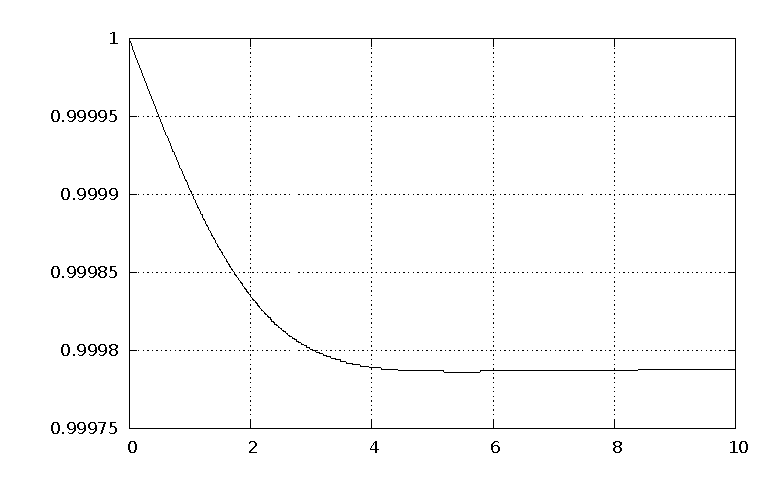
\includegraphics[width=.45\textwidth]
{figures/ellipse_both_bulk_inner_volume.ps}}
\subfloat[$\gamma\,\mathcal{H}^{1}(\Gamma^m)$]{
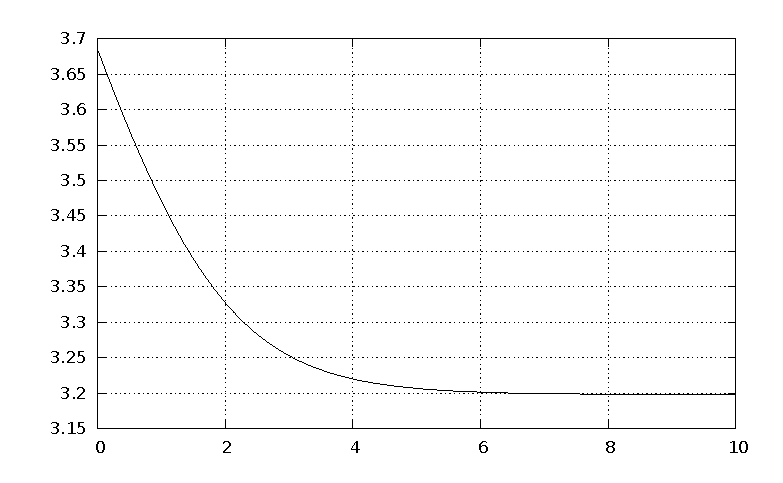
\includegraphics[width=.45\textwidth]
{figures/ellipse_both_interface_length.ps}}
\caption{Evolutions of the relative inner area and the interface energy for
the simulation in Figure~\ref{fig:ellipse_both}.}
\label{fig:ellipse_both_volumes}
\end{figure}
As a comparison, we show in Figure~\ref{fig:ellipse_smooth} the final snapshot
of the same simulation when no remeshings are performed, i.e.\ we use $C_r=
\infty$ in (\ref{eq:remesh}). We clearly see that due to the strong deformation
of the interface, this leads to elongated elements in the inner and in the
outer phase of the bulk finite element mesh.
\begin{figure}[htbp]
\centering
\subfloat[$t=10$]{\includegraphics[width=.32\textwidth]
{figures/ellipse_smooth_1000.ps}}
\caption{($\mu=\gamma=1$) Final pressure solution for a simulation as in
Figure~\ref{fig:ellipse_both}, when no remeshings are performed.}
\label{fig:ellipse_smooth}
\end{figure}

\subsection{Shear flow experiment in 2d}
As the final 2d numerical simulation we present a shear flow experiment
in the domain $\Omega=(-1,1)^2$, with a circle of radius $r=0.5$ as the
initial interface. Here we prescribe the inhomogeneous Dirichlet boundary
condition
\begin{equation*}
\vec g(\vec z)=(z_2,0)^T\quad \mbox{on }\partial\Omega\,,
\end{equation*}
and we use the parameters $\mu=1$, $\gamma=3$, $\tau=10^{-2}$ and $T=5$.
The initial interface is discretized with $J_\Gamma = 64$ surface elements,
and the initial bulk mesh has $J_\Omega^0 = 4240$ elements. In
Figure~\ref{fig:shear_2d} we show the evolution of the discrete pressures
for a simulation with $C_r=3$ for the P2--P0 element, while the velocities
are visualized in Figure~\ref{fig:shear_2d_velocity}.
\begin{figure}[htbp]
\centering
\subfloat[$t=0.5$]{
\includegraphics[width=.32\textwidth]{figures/2d_shear_050.ps}}
\subfloat[$t=1$]{
\includegraphics[width=.32\textwidth]{figures/2d_shear_100.ps}}
\subfloat[$t=5$]{
\includegraphics[width=.32\textwidth]{figures/2d_shear_500.ps}}
\caption{($\mu=1,\gamma=3$) Pressure evolution for the 2d shear flow with
$C_r=3$ for the P2--P0 element, uniform mesh.}
\label{fig:shear_2d}
\end{figure}

\begin{figure}[htbp]
\centering
\subfloat[$t=0.5$]{
\includegraphics[width=.32\textwidth]{figures/2d_shear_velocity_050.ps}}
\subfloat[$t=1$]{
\includegraphics[width=.32\textwidth]{figures/2d_shear_velocity_100.ps}}
\subfloat[$t=5$]{
\includegraphics[width=.32\textwidth]{figures/2d_shear_velocity_500.ps}}
\caption{($\mu=1,\gamma=3$) Velocity vector field for the 2d shear flow with
$C_r=3$ for the P2--P0 element, uniform mesh.}
\label{fig:shear_2d_velocity}
\end{figure}

\subsection{Convergence test in 3d} \label{sec:45}
Similarly to \S\ref{sec:41}, we perform the following convergence test for a
stationary spherical bubble in 3d. Let $\Omega = (-1,1)^3$ and
$\mu = \gamma = 1$. Then the true solution (\ref{eq:radialr},b) reduces to
$r(t) = \frac{1}{2}$, $\vec u(\cdot, t) = \vec 0$ and
$p(t) = 4\,\charfcn{\Omega_-(0)} - \frac{\pi}{12}$ for all $t\geq0$. We
approximate this stationary solution on nearly uniform meshes that feature
$J_\Gamma = 32$, $220$ and $596$ interface elements, and
$J_\Omega^0 = 408$, $3590$ and $20473$ bulk elements, respectively. Here, in
contrast to the situation in 2d, we are not able to define $\Gamma^0$
such that the vertices of $\Gamma^0$ lie on $\Gamma(0)$ and such that
(\ref{eq:constcurv}) is satisfied. As we would like to demonstrate the ability
of our method to recover the discrete stationary solution (\ref{eq:solsol})
also in 3d, we choose the initial interface $\Gamma^0$ such that
(\ref{eq:constcurv}) holds, at the expense of a nonzero initial error
$\| \Gamma^0 - \Gamma(0) \|_{L^\infty}$, recall (\ref{eq:errorXx}). We obtain
such an initial triangulation with the help of the numerical scheme from
\cite{gflows3d} for surface diffusion, which is a gradient flow for
surface area that maintains the enclosed volume. See
e.g.\ \cite[Fig.\ 11]{gflows3d} for an evolution towards a polyhedral
approximation of a sphere that satisfies (\ref{eq:constcurv}), and hence also
(\ref{eq:conformal}). We report the
errors for the P2--P0 element in Table~\ref{tab:bubble3Dp2p0}, while
Table~\ref{tab:bubble3Dp2p1p0} shows the same errors for the P2--(P1+P0)
element. In both cases we use the uniform time step size $\tau = 10^{-2}$.
\begin{table*}
\center
\begin{tabular}{rlllr}
\hline
$J_\Gamma$ & $\errorXx$ & $\errorUu2$ & $\LerrorPp$ & $CPU[s]$ \\
\hline
 32 & 2.97986e-02 & 0 & 1.65555e-00 &   385 \\
220 & 5.80971e-03 & 0 & 7.14269e-01 &  4699 \\
596 & 2.42857e-03 & 0 & 3.58466e-01 & 51604 \\
\hline
\end{tabular}
\caption{($\mu=\gamma=1$) Stationary bubble problem on $(-1,1)^3$ over the time
interval $[0,1]$ for the P2--P0 element.}
\label{tab:bubble3Dp2p0}
\end{table*}

\begin{table*}
\center
\begin{tabular}{rlllr}
\hline
$J_\Gamma$ & $\errorXx$ & $\errorUu2$ & $\LerrorPp$ & $CPU[s]$ \\
\hline
 32 & 2.97986e-02 & 0 & 1.65749e-00 &   568 \\
220 & 5.80971e-03 & 0 & 7.15353e-01 &  9174 \\
596 & 2.42857e-03 & 0 & 3.59181e-01 & 121110 \\
\hline
\end{tabular}
\caption{($\mu=\gamma=1$) Stationary bubble problem on $(-1,1)^3$ over the time
interval $[0,1]$ for the P2--(P1+P0) element.}
\label{tab:bubble3Dp2p1p0}
\end{table*}

We note that we again recover the discrete stationary solutions
(\ref{eq:solsol}). Here this leads to a nonzero error in the position of the
discrete interface, because the vertices of the initial interface $\Gamma^0$ do
not lie on $\Gamma(0)$.

\subsection{Shear flow experiment in 3d}
Finally, we also report on a shear flow experiment in the domain
$\Omega=(-1,1)^3$, with a sphere of radius $r=0.5$ as the initial interface.
The initial interface mesh has $J_\Gamma = 596$ elements, while the nearly
uniform bulk mesh is made up of $J_\Omega^0 = 19641$ elements. We prescribe the
inhomogeneous Dirichlet boundary condition
\begin{equation*}
\vec g(\vec z)=(z_3,0,0)^T\quad \mbox{on }\partial\Omega\,,
\end{equation*}
and we use the parameters $\mu=1$, $\gamma=3$, $\tau=10^{-2}$ and $T=5$.
In Figure~\ref{fig:shear_3d} we show the evolution of the discrete interface
for a simulation with $C_r=3$ for the P2--P0 element, while the velocities
are visualized in Figure~\ref{fig:shear_3d_velocity}.
\begin{figure}[htbp]
\centering
\subfloat[$t=0$]{
\includegraphics[width=.32\textwidth]{figures/3d_shear_000.ps}}
\subfloat[$t=1$]{
\includegraphics[width=.32\textwidth]{figures/3d_shear_100.ps}}
\subfloat[$t=5$]{
\includegraphics[width=.32\textwidth]{figures/3d_shear_500.ps}}
\caption{($\mu=1,\gamma=3$) Interface evolution for the 3d shear flow with
$C_r=3$ for the P2--P0 element, uniform mesh.}
\label{fig:shear_3d}
\end{figure}

\begin{figure}[htbp]
\centering
\subfloat[$t=1$]{
\includegraphics[width=.32\textwidth]{figures/3d_shear_velocity_100.ps}}
\subfloat[$t=5$]{
\includegraphics[width=.32\textwidth]{figures/3d_shear_velocity_500.ps}}
\caption{($\mu=1,\gamma=3$) Velocity vector field in the plane normal to
$(0,1,0)^T$ and passing through the origin for the 3d shear flow with $C_r=3$
for the P2--P0 element, uniform mesh.}
\label{fig:shear_3d_velocity}
\end{figure}
A plot of the relative inner volume over time is shown in
Figure~\ref{fig:shear_3d_bulk_inner_volume}, where we again observe that our
numerical method maintains the enclosed volume well.

\begin{figure}[htbp]
\centering
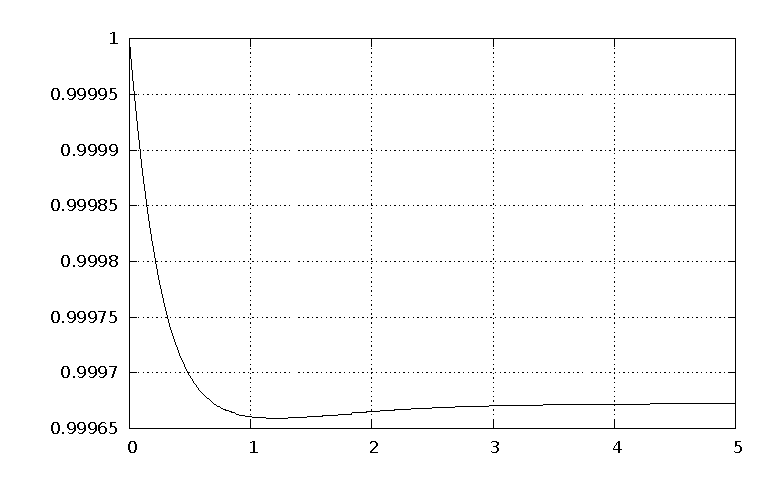
\includegraphics[width=.45\textwidth]{figures/3d_shear_bulk_inner_volume.ps}
\caption{A plot of the relative inner volume
$\frac{\mathcal{L}^3(\Omega^m_-)}{\mathcal{L}^3(\Omega^0_-)}$
over time for the simulation in Figure~\ref{fig:shear_3d}.}
\label{fig:shear_3d_bulk_inner_volume}
\end{figure}

\section{Conclusion}\label{sec:conclusion}
We have presented a novel fitted finite element approximation for two-phase
Stokes flow. The method uses a piecewise linear approximation of the interface
and employs standard velocity and pressure finite element spaces in the bulk.

The scheme is unconditionally stable and can capture simple stationary
solutions exactly, which means that no spurious velocities appear. In addition,
the discontinuous pressure jumps are captured well in general situations, and
no pressure oscillations appear in practice.

Moreover, the numerical solutions exhibit good volume conservation properties
and the quality of the interface mesh does not deteriorate in time.

\bibliographystyle{siam}
\bibliography{../bib/robert_refs,../bib/marco_refs}
\end{document}
